Trong mô hình khách hàng - nhà cung cấp, nếu nhà cung cấp thực hiện tốt yêu cầu thì khách hàng cần tuân thủ chặt chẽ. Mô hình tuân thủ (Conformist) là một mối quan hệ trong đó bối cảnh bị giới hạn hạ lưu áp dụng mô hình, ngôn ngữ chung và các khái niệm của bối cảnh bị giới hạn thượng nguồn.

Trong mô hình tuân thủ bối cảnh bị giới hạn hạ lưu được ký hiệu là CF.

%! $VD: - - >

%! $VD: A - CF - U - B - - >

%! $VD: A - users(id, name) - B cũng users(id, name) - - >

% Vẽ lại bản đồ tiếng Việt

% Vẽ lại bản đồ tiếng Việt

% Vẽ lại bản đồ tiếng Việt

% Vẽ lại bản đồ tiếng Việt

% Vẽ lại bản đồ tiếng Việt

% Vẽ lại bản đồ tiếng Việt

% Vẽ lại bản đồ tiếng Việt

% Vẽ lại bản đồ tiếng Việt

% Từ bản đồ lấy vi dụ cho các mô hình

% Từ bản đồ lấy vi dụ cho các mô hình

% Từ bản đồ lấy vi dụ cho các mô hình

% Từ bản đồ lấy vi dụ cho các mô hình

% Từ bản đồ lấy vi dụ cho các mô hình

% Từ bản đồ lấy vi dụ cho các mô hình

% Từ bản đồ lấy vi dụ cho các mô hình

% Từ bản đồ lấy vi dụ cho các mô hình

% Từ bản đồ lấy vi dụ cho các mô hình

% Từ bản đồ lấy vi dụ cho các mô hình

\begin{example} Trong miền vấn đề ngân hàng, thẻ tín dụng và khoản vay mua nhà không có mối quan hệ.

\begin{figure}[H]

\centering

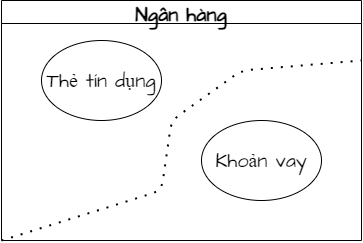
\includegraphics[scale = 0.5]{pictures/mo_hinh_rieng_biet_separate_ways/main.drawio.png}

\caption{Ví dụ mô hình riêng biệt (Separate Ways)}

\end{figure}

\end{example}

